\chapter{Interfaces with \dword{lbnf}}
\label{vl:tc-lbnf}

\section{Organization of Interfaces}
\label{sec:inter-org-interf}
To manage interfaces within the detector and between the
detector and facilities, an overall integration mechanism has been
developed consisting of integration nodes. Each node is integrated
and managed by a specific group. The interfaces between the nodes are
managed by the \dword{tc} engineering team.

Figure~\ref{fig:integration_nodes} shows the interfaces between the
detector and facilities.
\begin{dunefigure}[Integration Nodes.]{fig:integration_nodes}
  {Overall integration nodes and interfaces.}
  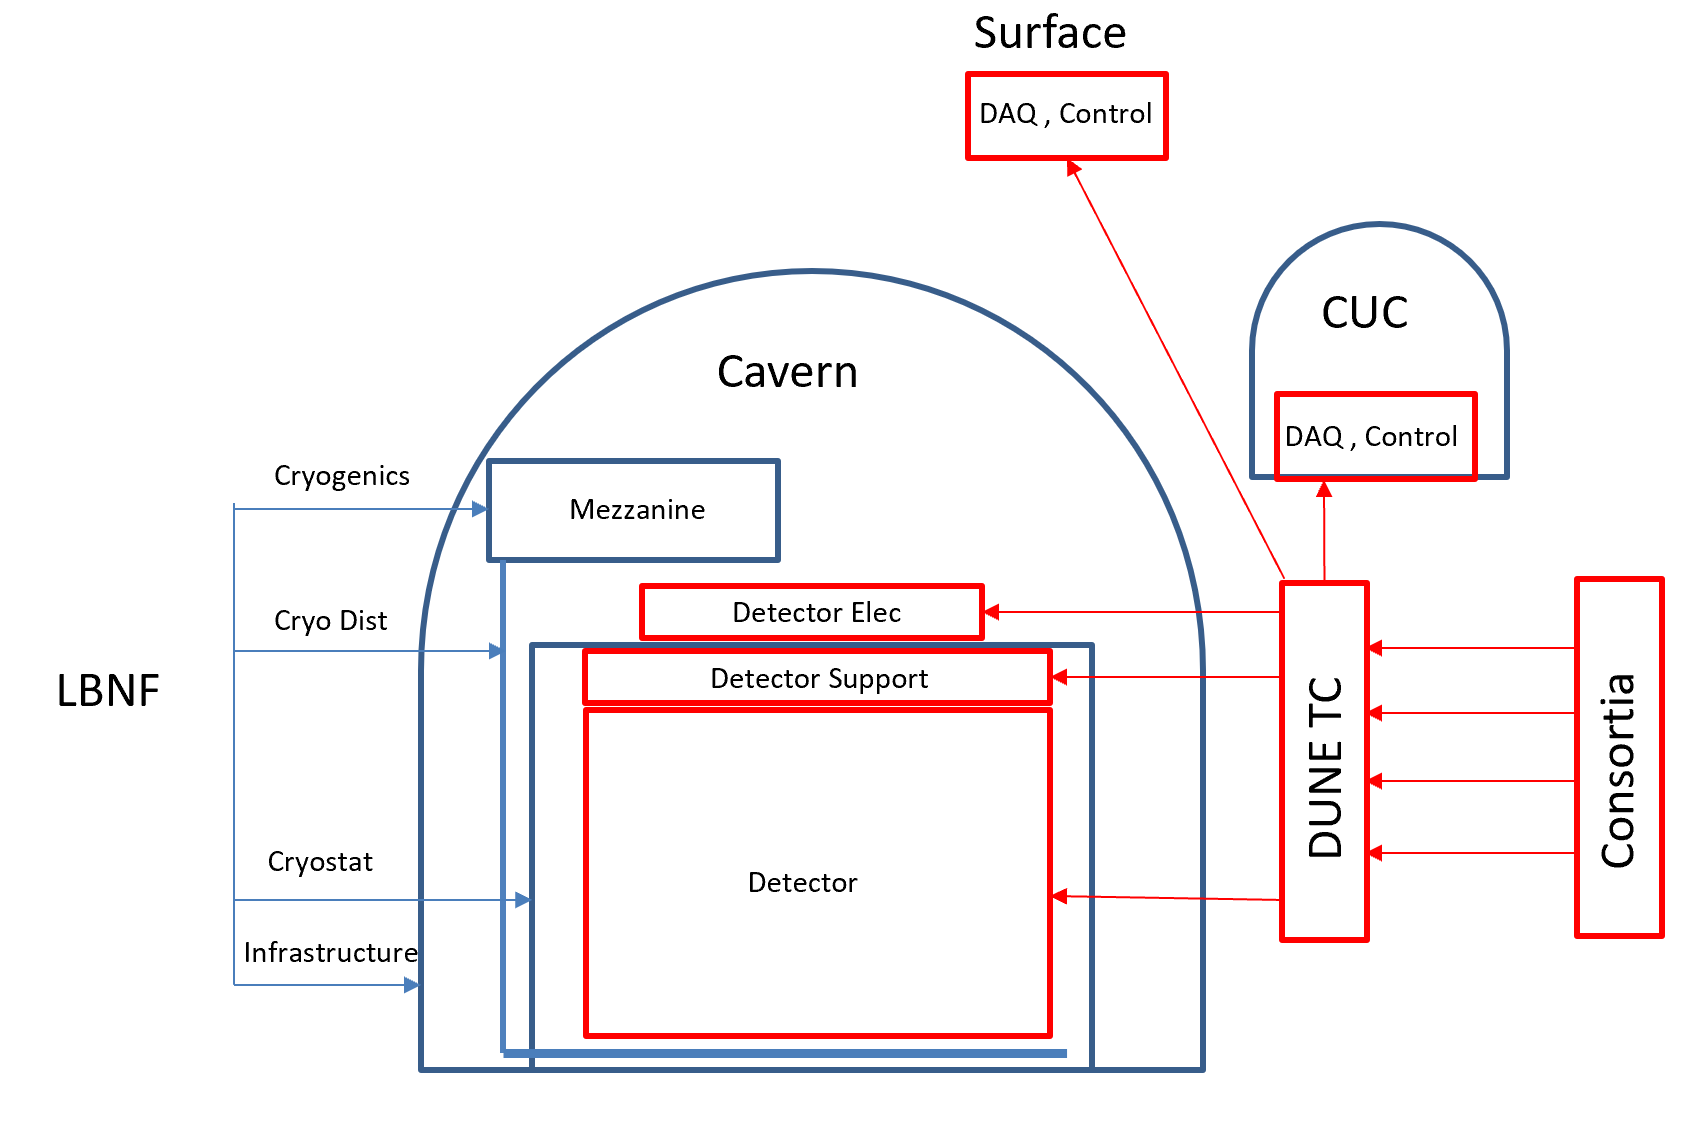
\includegraphics[width=0.7\textwidth]{Integration_nodes.png}
\end{dunefigure}
In the figure, within the cavern, items provided by \dword{lbnf} are
on the left and the items provided by \dword{dune} are on the right. In addition, the \dword{tc} engineering team integrates the \dword{daq} room in the central utility
cavern and surface control and network rooms. Interfaces with \dword{lbnf} are
managed at the boundaries of each integration node. As an example, the
interface between \dword{lbnf} and \dword{dune} for the underground \dword{daq} and control
rooms are power, cooling water, data fibers and cable penetrations at the
room boundaries. Implementing power, cooling water, data, and
signal cables as well as integrating the racks are the responsibilities of \dword{dune}.


The integration nodes comprise the following:
\begin{itemize}
\item {\bf Detector:} This consists of all \dword{tpc} elements within
  the \dword{lar}. Almost all consortia are involved in this
  integration task, which is mostly mechanical. Consortia engineering
  teams work directly with the \dword{tc} engineering team.  The
  primary interface is with \dword{dss} through hangers. Examples of
  interfaces within this node include: \dword{fc} connections to both
  \dwords{cpa} and \dwords{apa}, \dword{ce} and \dword{pd} cable
  routing within the cryostat and location of calibration and
  cryogenic instrumentation.
  \item {\bf \dword{dss}:} This consists of all detector support elements,
  cable trays and feedthroughs.
\item {\bf Detector Electronics:} This consists of all racks, cooling, power, cable
  trays, cable distribution on top of cryostats, rack protection
  (smoke detectors, hardware power trip), rack component build and the interface to
  the \dword{ddss}.
\item {\bf \dword{daq} and Electronics:} This includes electronics on top of cryostat,
  in the \dword{daq} room and in the surface rooms. This also includes the  fiber optic distribution from
  the surface to the \dword{daq} room and teh fiber optic distribution from the
  detectors to the \dword{daq} room. It also includes the layout and cooling of the \dword{daq}
  room.
\end{itemize}

\section{Interfaces with \dword{lbnf}}
\label{sec:inter-lbnf-interf}
The following figures and explanations show the
integration of the detector modules within the cavern. The interface
boundaries are not specifically pointed out in each figure, but they
follow the scheme as represented in
Figure~\ref{fig:integration_nodes}.

Figure~\ref{fig:detector_cavern} shows one detector module in the
cavern. In this figure, the cryogenics equipment and racks on top of
the detector are visible. The \dword{lar} recirculation pumps can also be seen
on the lower level.
\begin{dunefigure}[Overall view of the detector in cavern.]{fig:detector_cavern}
  {Overall view of a detector module within the cavern.}
  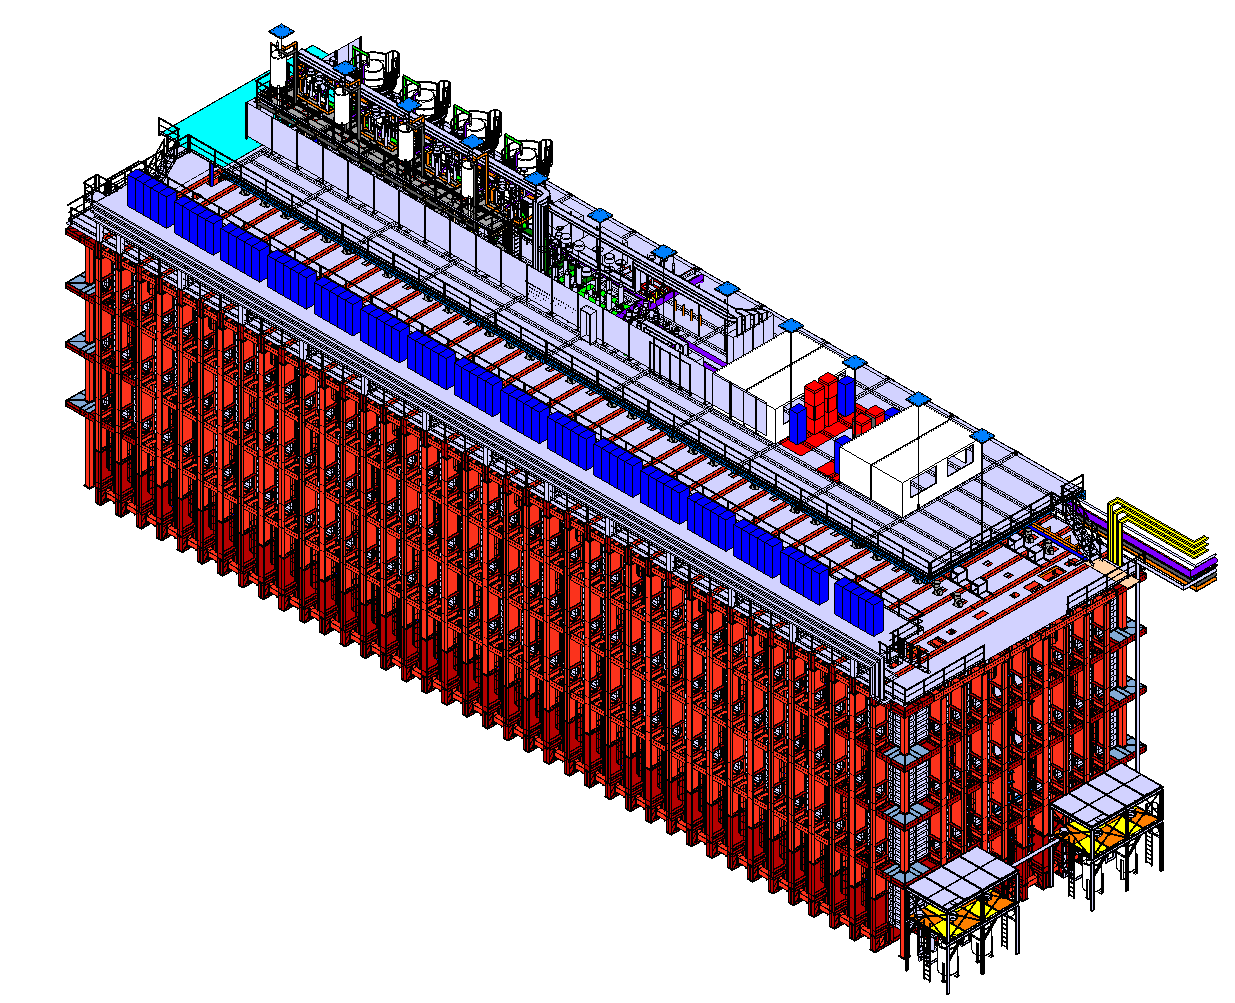
\includegraphics[width=0.8\textwidth]{LBNF-Cryostat-NW_Iso_c.png}
\end{dunefigure}

Figure~\ref{fig:detector_ew_elevation} shows the east to west elevation view of the
detector in the cavern. The services from the
\dword{cuc} enter the cavern through a passage visible on the left.
\begin{dunefigure}[East-west elevation view of Detector]{fig:detector_ew_elevation}
  {East-west elevation view of one detector module in the cavern.}
  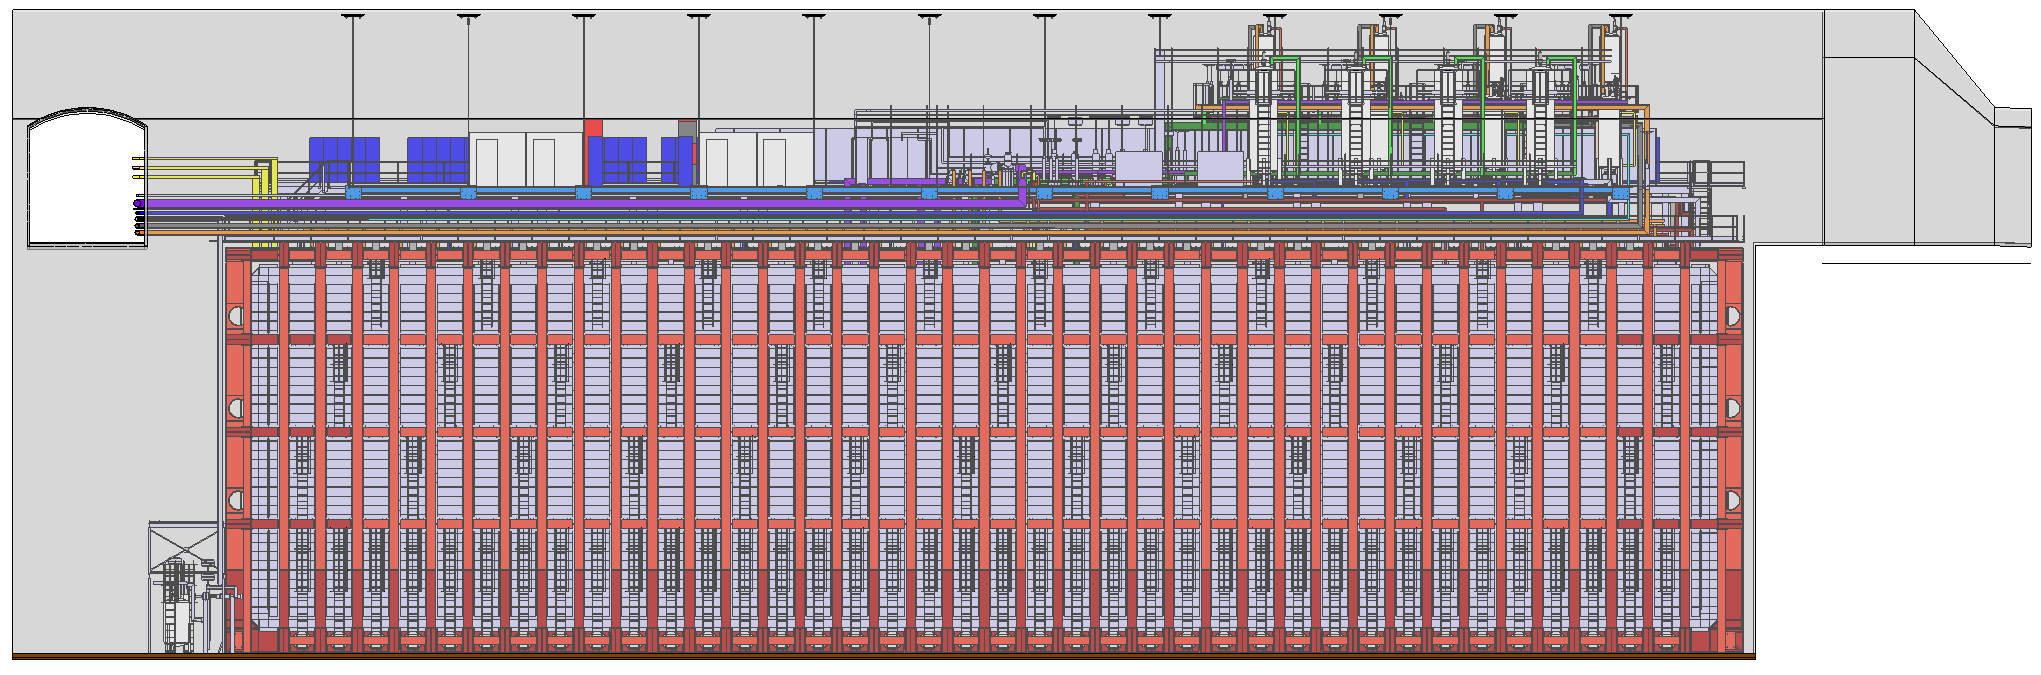
\includegraphics[width=0.9\textwidth]{LBNF-Cryostat-South_Elevation_in_Cavern_c.png}
\end{dunefigure}

Figure~\ref{fig:detector_ns_elevation} shows the north to south elevation view of the
detector in the cavern. The services entering
from the \dword{cuc} are visible on the right.
\begin{dunefigure}[North-south elevation view of detector]{fig:detector_ns_elevation}
  {North-south elevation view of one detector in the cavern.}
  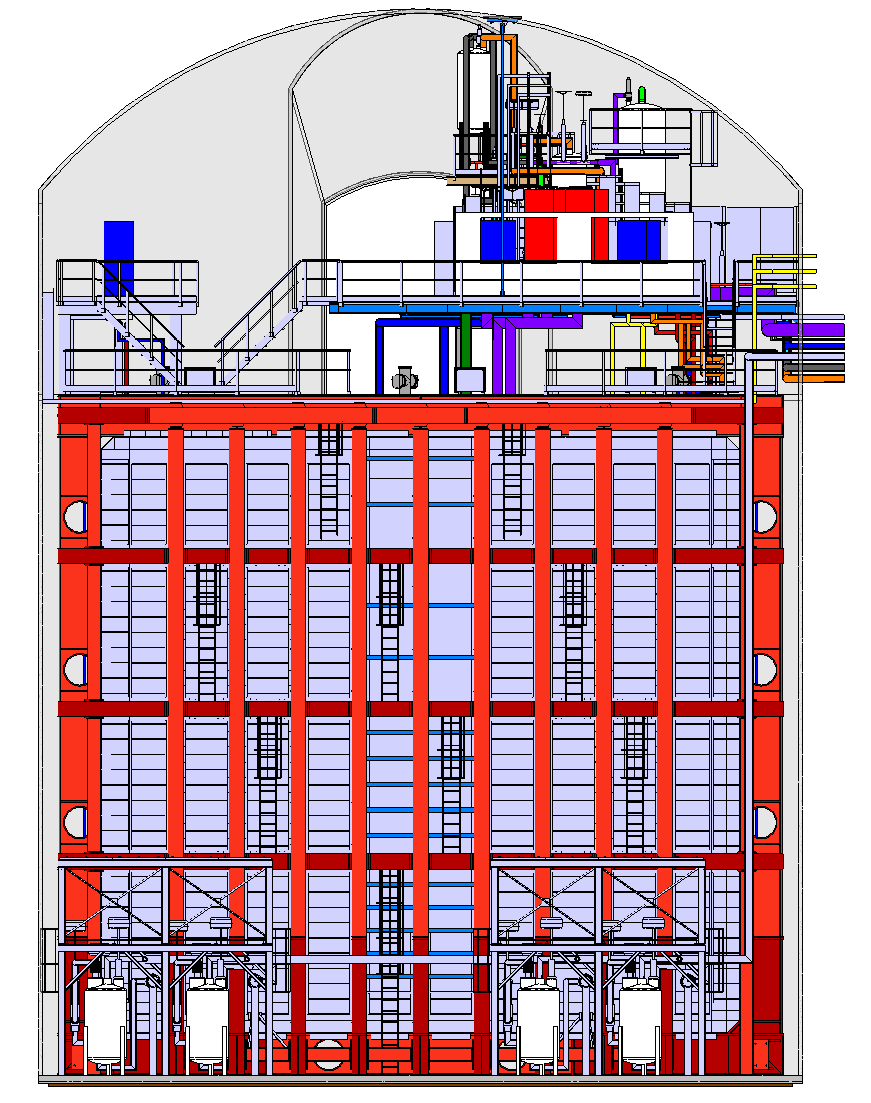
\includegraphics[width=0.7\textwidth]{LBNF-Cryostat-West_Elevation_in_Cavern_c.png}
\end{dunefigure}

Figure~\ref{fig:detector_mezzanines} shows the elevation view of the
top of cryostat showing mezzanines, cryogenic equipment, and electronic
racks.
\begin{dunefigure}[Elevation view of top of cryostat showing mezzanines, cryogenic
    equipment and electronic racks.]{fig:detector_mezzanines}
  {Elevation view of top of cryostat showing mezzanines, cryogenic
    equipment, and electronic racks.}
  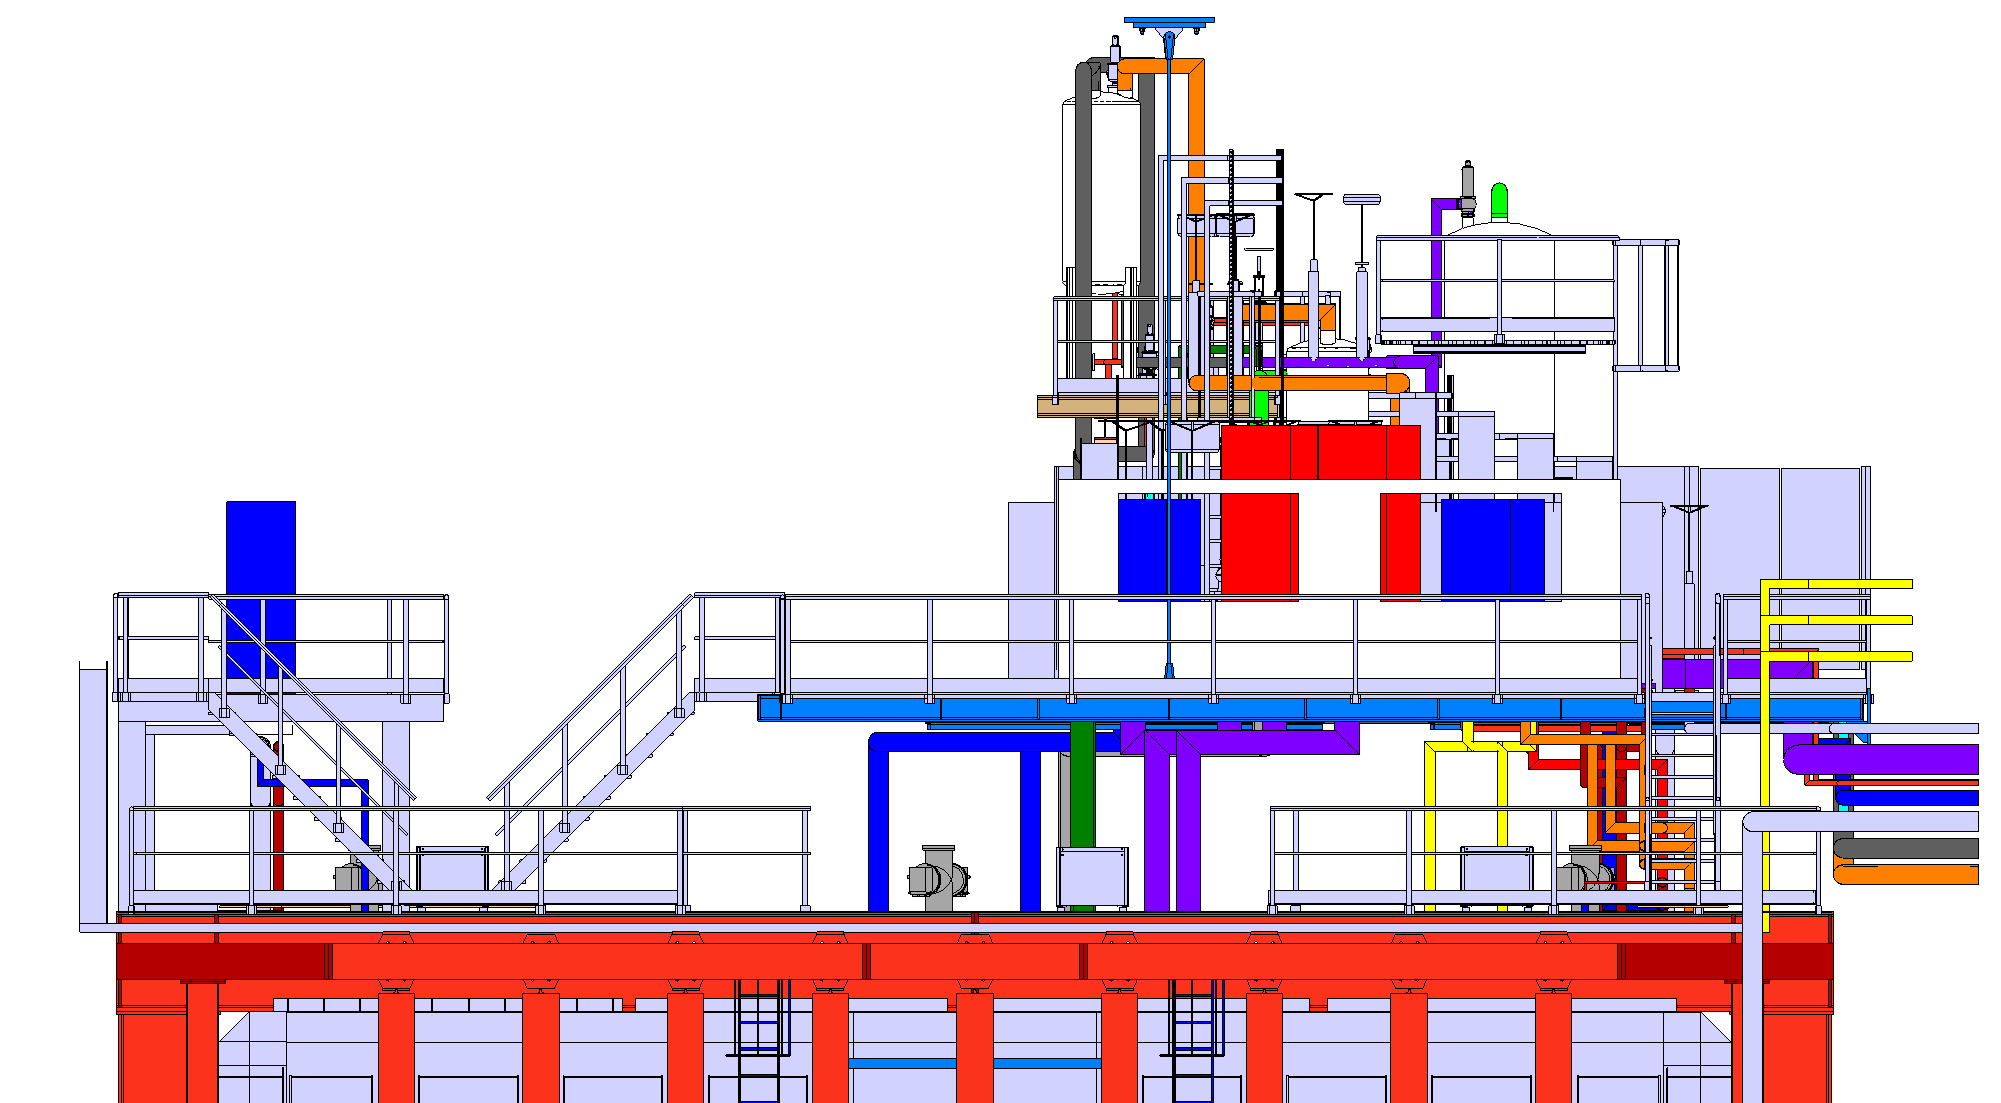
\includegraphics[width=0.85\textwidth]{LBNF-Cryostat-West_Elevation-Cryo_c.png}
\end{dunefigure}
The cryogenics are installed on a mezzanine supported from
the cavern roof and cavern wall. Cryogenic distribution lines are
routed under the mezzanine. Local control rooms for the
cryogenic equipment are on the mezzanine.

Detector electronics are installed in short racks close to
feedthroughs and in taller racks installed on a separate electronics
mezzanine shown on the left of Fig.~\ref{fig:detector_mezzanines}.
This will allow easy access for maintenance and reduce complexity on
top of the detector.
